\documentclass{article}

\usepackage{booktabs}
\usepackage{fancyhdr}
\usepackage{float}
\usepackage{graphicx}
\usepackage{helvet}
\usepackage{hyperref}
\usepackage{tabularx}
\usepackage{xcolor}

\usepackage{framed}     % These needed for the code formatter
\usepackage{color}
\usepackage{fancyvrb}

\usepackage{makeidx}         % allows index generation
\makeindex

% Use helvetica (sans) by default
\renewcommand{\familydefault}{\sfdefault}

% Greenish links
\hypersetup{
  colorlinks=true,
  linkcolor=blue!50!red,
  urlcolor=green!70!black
}

\setlength{\parindent}{0pt}
\setlength{\parskip}{1em}

\makeatletter
\renewcommand{\@dotsep}{4.5}
\renewcommand{\l@section}{\@dottedtocline{1}{1.5em}{2.3em}}
\renewcommand{\l@subsection}{\@dottedtocline{2}{2.0em}{2.8em}}
\makeatother

\setlength{\headheight}{40pt}
\setlength{\headsep}{0.2in}

\pagestyle{fancy}
\lhead{\includegraphics[width=0.2\textwidth]{img/logo}}
\chead{TermDriver2 User Guide}
\rhead{\thepage}
\cfoot{\textcopyright \the\year \ \ Excamera Labs}
\renewcommand{\headrulewidth}{0.5pt}
\renewcommand{\footrulewidth}{0.5pt}

\usepackage{array}
\newcolumntype{L}[1]{>{\raggedright\let\newline\\\arraybackslash\hspace{0pt}}m{#1}}
\newcolumntype{C}[1]{>{\centering\let\newline\\\arraybackslash\hspace{0pt}}m{#1}}
\newcolumntype{R}[1]{>{\raggedleft\let\newline\\\arraybackslash\hspace{0pt}}m{#1}}

\newcommand{\heavyline}{\specialrule{1pt}{1pt}{1pt}}
\newcommand{\png}[2]{
\begin{figure}[H]
\begin{center}
\includegraphics[width=0.75\textwidth]{#1}
\caption{#2}
\end{center}
\end{figure}
}

\newcommand{\mach}[1]{\texttt{\textbf{#1}}}
\newcommand{\gap}{\vspace{10pt}}

\input{pyg.tex}

\begin{document}

\newpage
\begin{center}
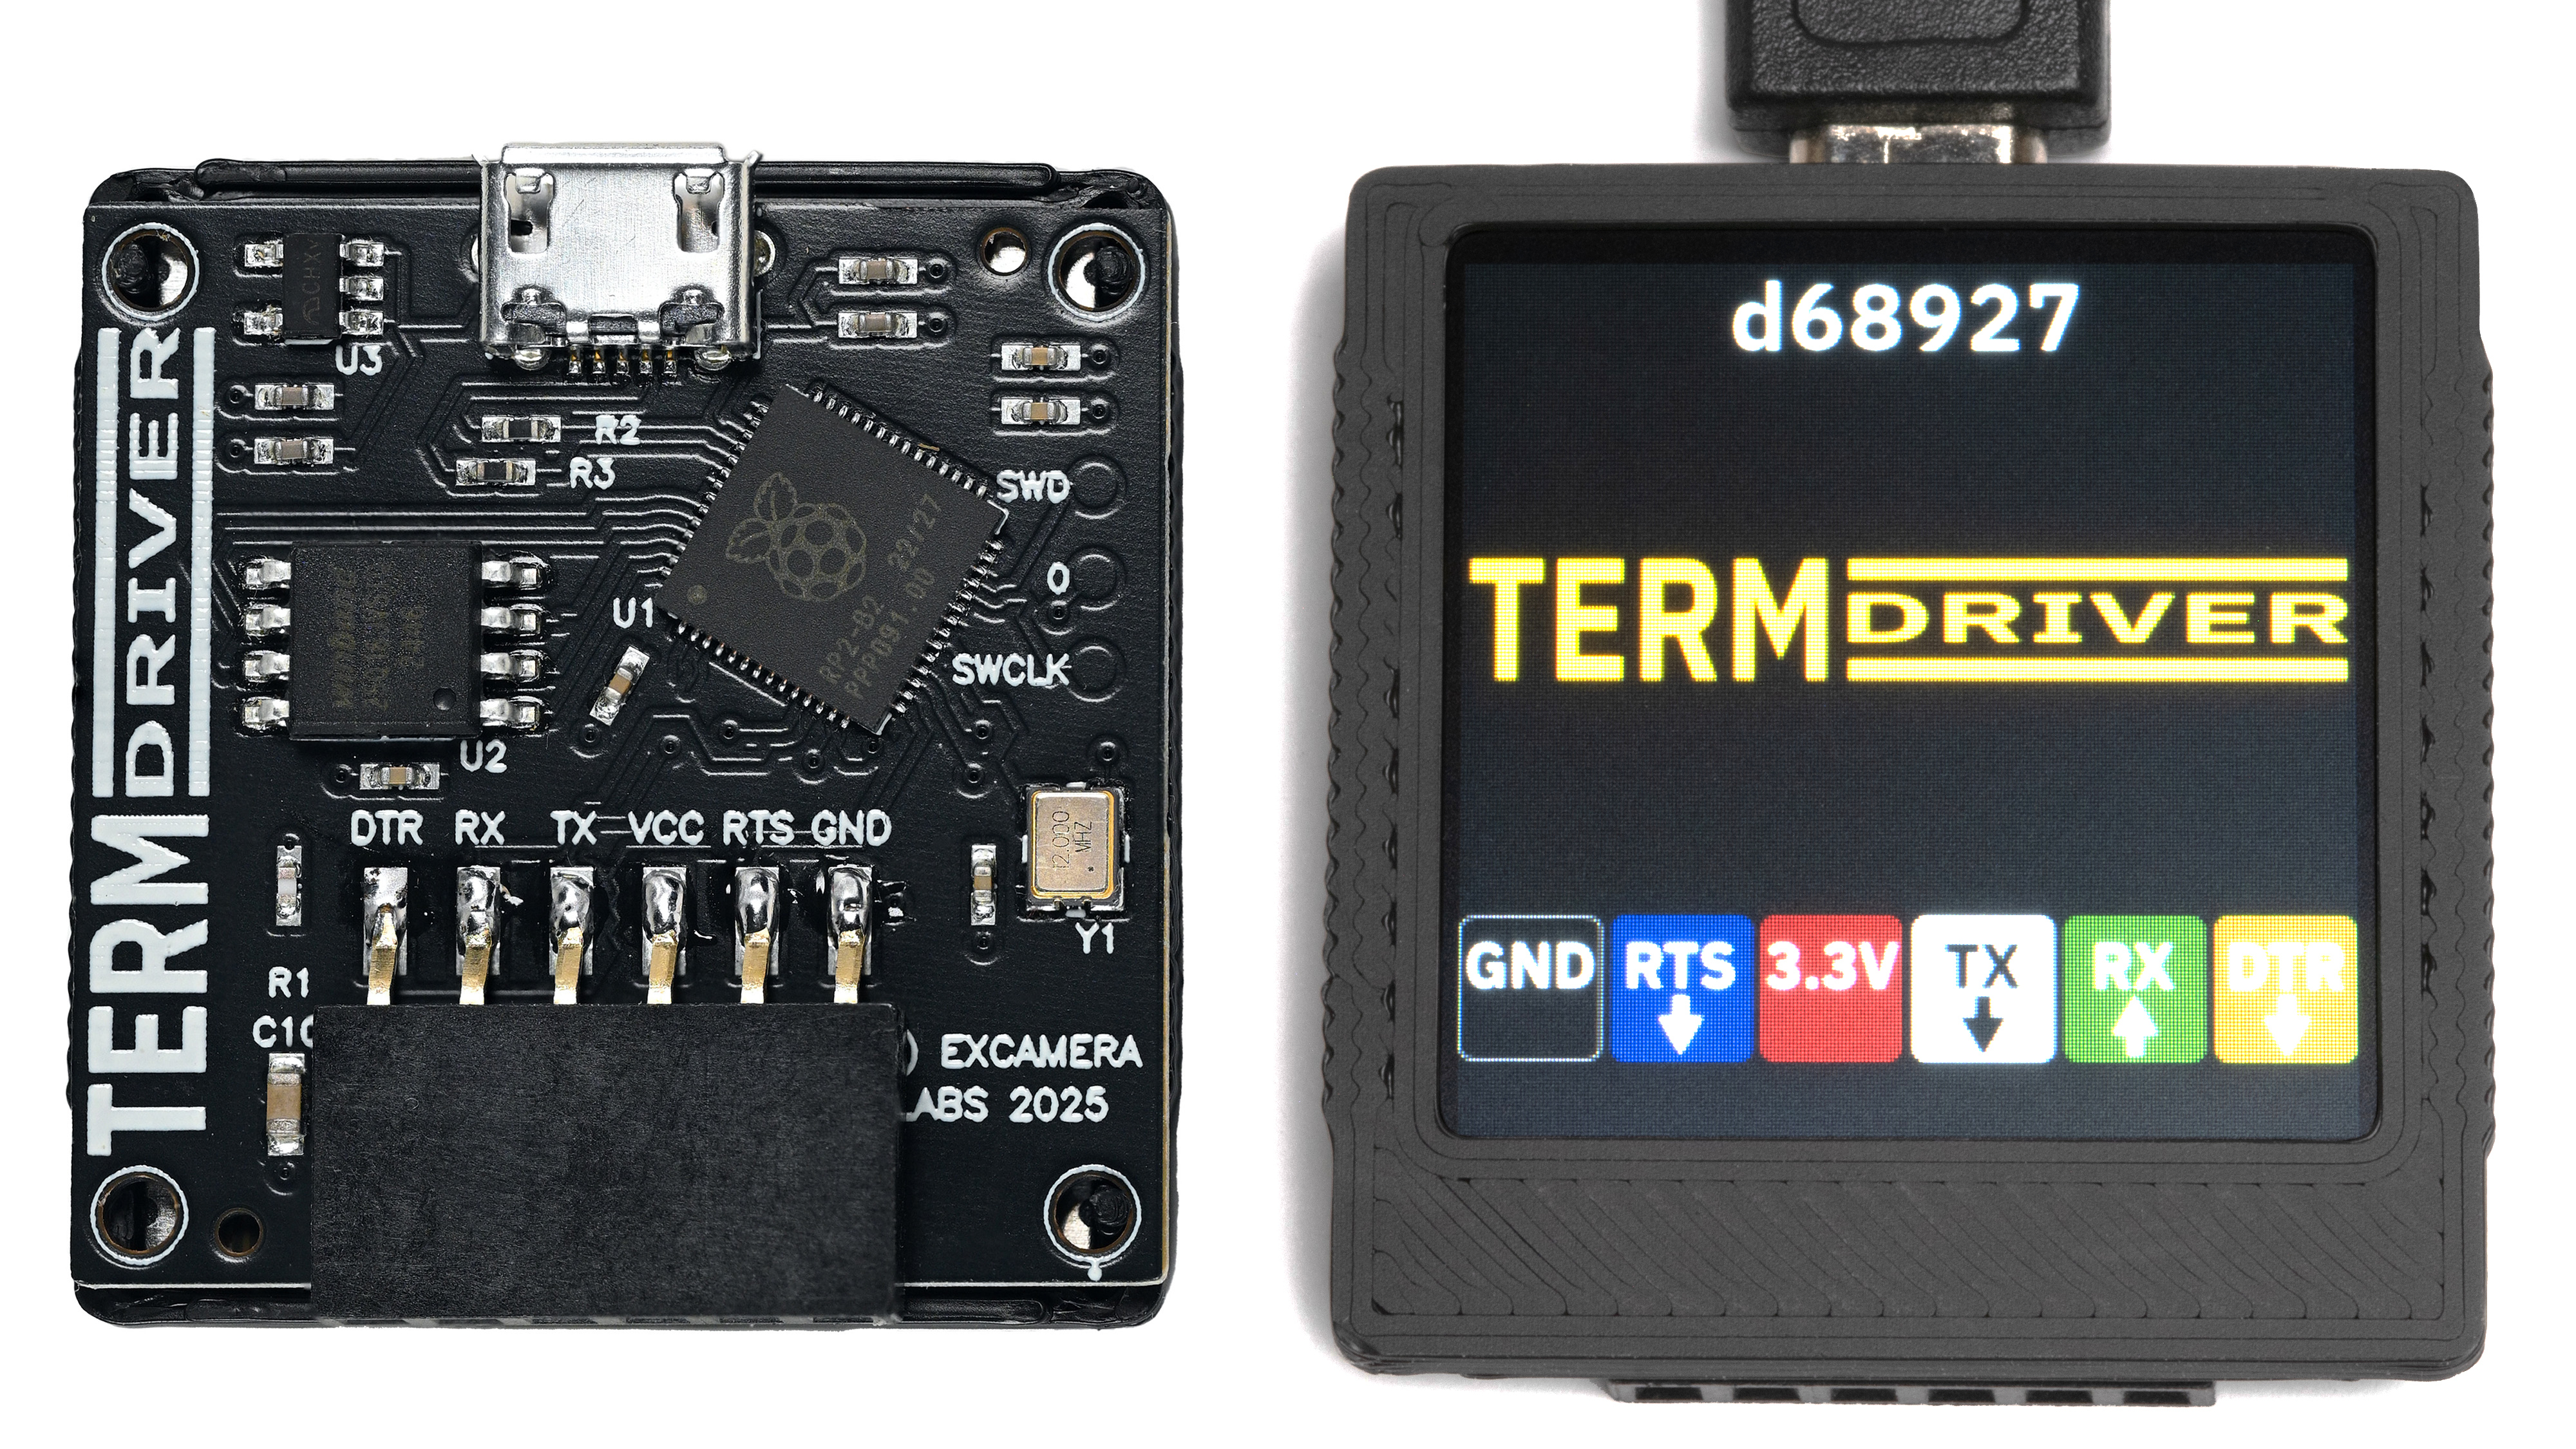
\includegraphics[width=0.75\textwidth]{img/termdriver2/termdriver2-front-back-01-comp}
\end{center}
\tableofcontents
% \listoffigures

\section{Overview}

TermDriver2 is a USB to serial adapter with a built-in screen.
All through traffic is displayed on the screen in real-time, together
with line protocol information.

\section{Features}
\begin{itemize}
\item support for serial rates from 110 to 2M baud
\item compact and bright 40x22 terminal display
\item full set of ANSI control codes supported
\item 32K receive buffer for robust reception even when the host PC is heavily loaded
\item 3.3 V output at up to 300 mA
\end{itemize}

\newpage
\section{Installation}

\begin{enumerate}
\item Connect a micro USB cable to the TermDriver 2
\item You should see the screen power up with the TermDriver logo and serial number
\item Confirm that the serial device is present on your host PC
\item Find the relevant port \index{port} on your host PC
\item Connect the serial outputs to your target device
\item Use the TermDriver as a USB to serial adapter
\end{enumerate}

\section{ANSI escape codes}\index{ANSI}

TermDriver2 implements the ANSI terminal
\href{https://en.wikipedia.org/wiki/ANSI_escape_code\#CSI_sequences}{control codes}.

\gap\noindent
\begin{tabularx}{\linewidth}{lX}
\heavyline
Code & Effect \\ \heavyline

ESC \mach{{[} \emph{n} A } & Cursor up \\

ESC \mach{{[} \emph{n} B } & Cursor down \\

ESC \mach{{[} \emph{n} C } & Cursor forward \\

ESC \mach{{[} \emph{n} D } & Cursor back \\

ESC \mach{{[} \emph{c} G } & Moves the cursor to column $c$ \\

ESC \mach{{[} \emph{r;c} H } & Moves the cursor to row $r$ column $c$ \\

ESC \mach{{[} \emph{n} J } & Erase display \\

ESC \mach{{[} \emph{n} l } & Erase display \\

ESC \mach{{[} \emph{n} m } & Select graphic rendition \\

ESC \mach{{[} 6n } & Reports the cursor position (CPR) by transmitting \mach{ESC[$n$;$m$R}, where n is the row and m is the column. \\

% ESC {[} s & Save cursor position \\

% ESC {[} u & Restore cursor position \\ \heavyline
\end{tabularx}
\gap

\noindent
Select graphic rendition (SGR) sets display attributes.
Suported sequences are:

\gap\noindent
\begin{tabularx}{\linewidth}{lX}
\heavyline
Code & Effect \\ \heavyline

0 & Normal: all attributes become turned off \\
8 & Conceal \\
30..37 & Set foreground color \\
38 & Set foreground color. Next arguments are \mach{5;n} or \mach{2;r;g;b} \\
39 & Default foreground color \\
40..47 & Set background color \\
48 & Set foreground color. Next arguments are \mach{5;n} or \mach{2;r;g;b} \index{color!RGB}\\
49 & Default background color \\

\end{tabularx}
\gap

In addition the following sequences are specific to TermDriver:

\gap
\noindent
\begin{tabularx}{\linewidth}{lX}
\heavyline
Code & Effect \\ \heavyline

ESC \mach{{[}7n} & Reports the 6 digit hex id of the TermDriver \\
ESC \mach{{[}1413829197;$id$;0l} & Reset to UF2 bootloader mode \\
ESC \mach{{[}1413829197;$id$;1l} & Reboot \\

\\ \heavyline
\end{tabularx}
\gap
Where $id$ is the 6 hex digit id of the TermDriver, as a decimal number.

\begin{center}
\includegraphics[width=0.5\textwidth]{img/termdriver2/termdriver2-front}
\end{center}

\noindent
For example if the TermDriver has id \mach{d68927}, then $id$ is 14059815,
and the sequence to enter UF2 bootloader mode is:

\begin{verbatim}
ESC [ 1413829197;14059815;0
\end{verbatim}

After entering UF2 \index{UF2} mode,
the TermDriver's firmware appears as a drive on the host PC named \mach{RPI-RP2}.
New firmware can be copied into the file, and when complete, the TermDriver will reboot
and run the new firmware. \index{firmware}

There is a Python program in \mach{demos/reset\_to\_uf2.py} in the
\href{https://github.com/jamesbowman/termdriver2}{TermDriver 2 respository}
that uses these commands to put the TermDriver 2 into UF2 bootloader mode.

\newpage
\section{Hardware}

\begin{center}
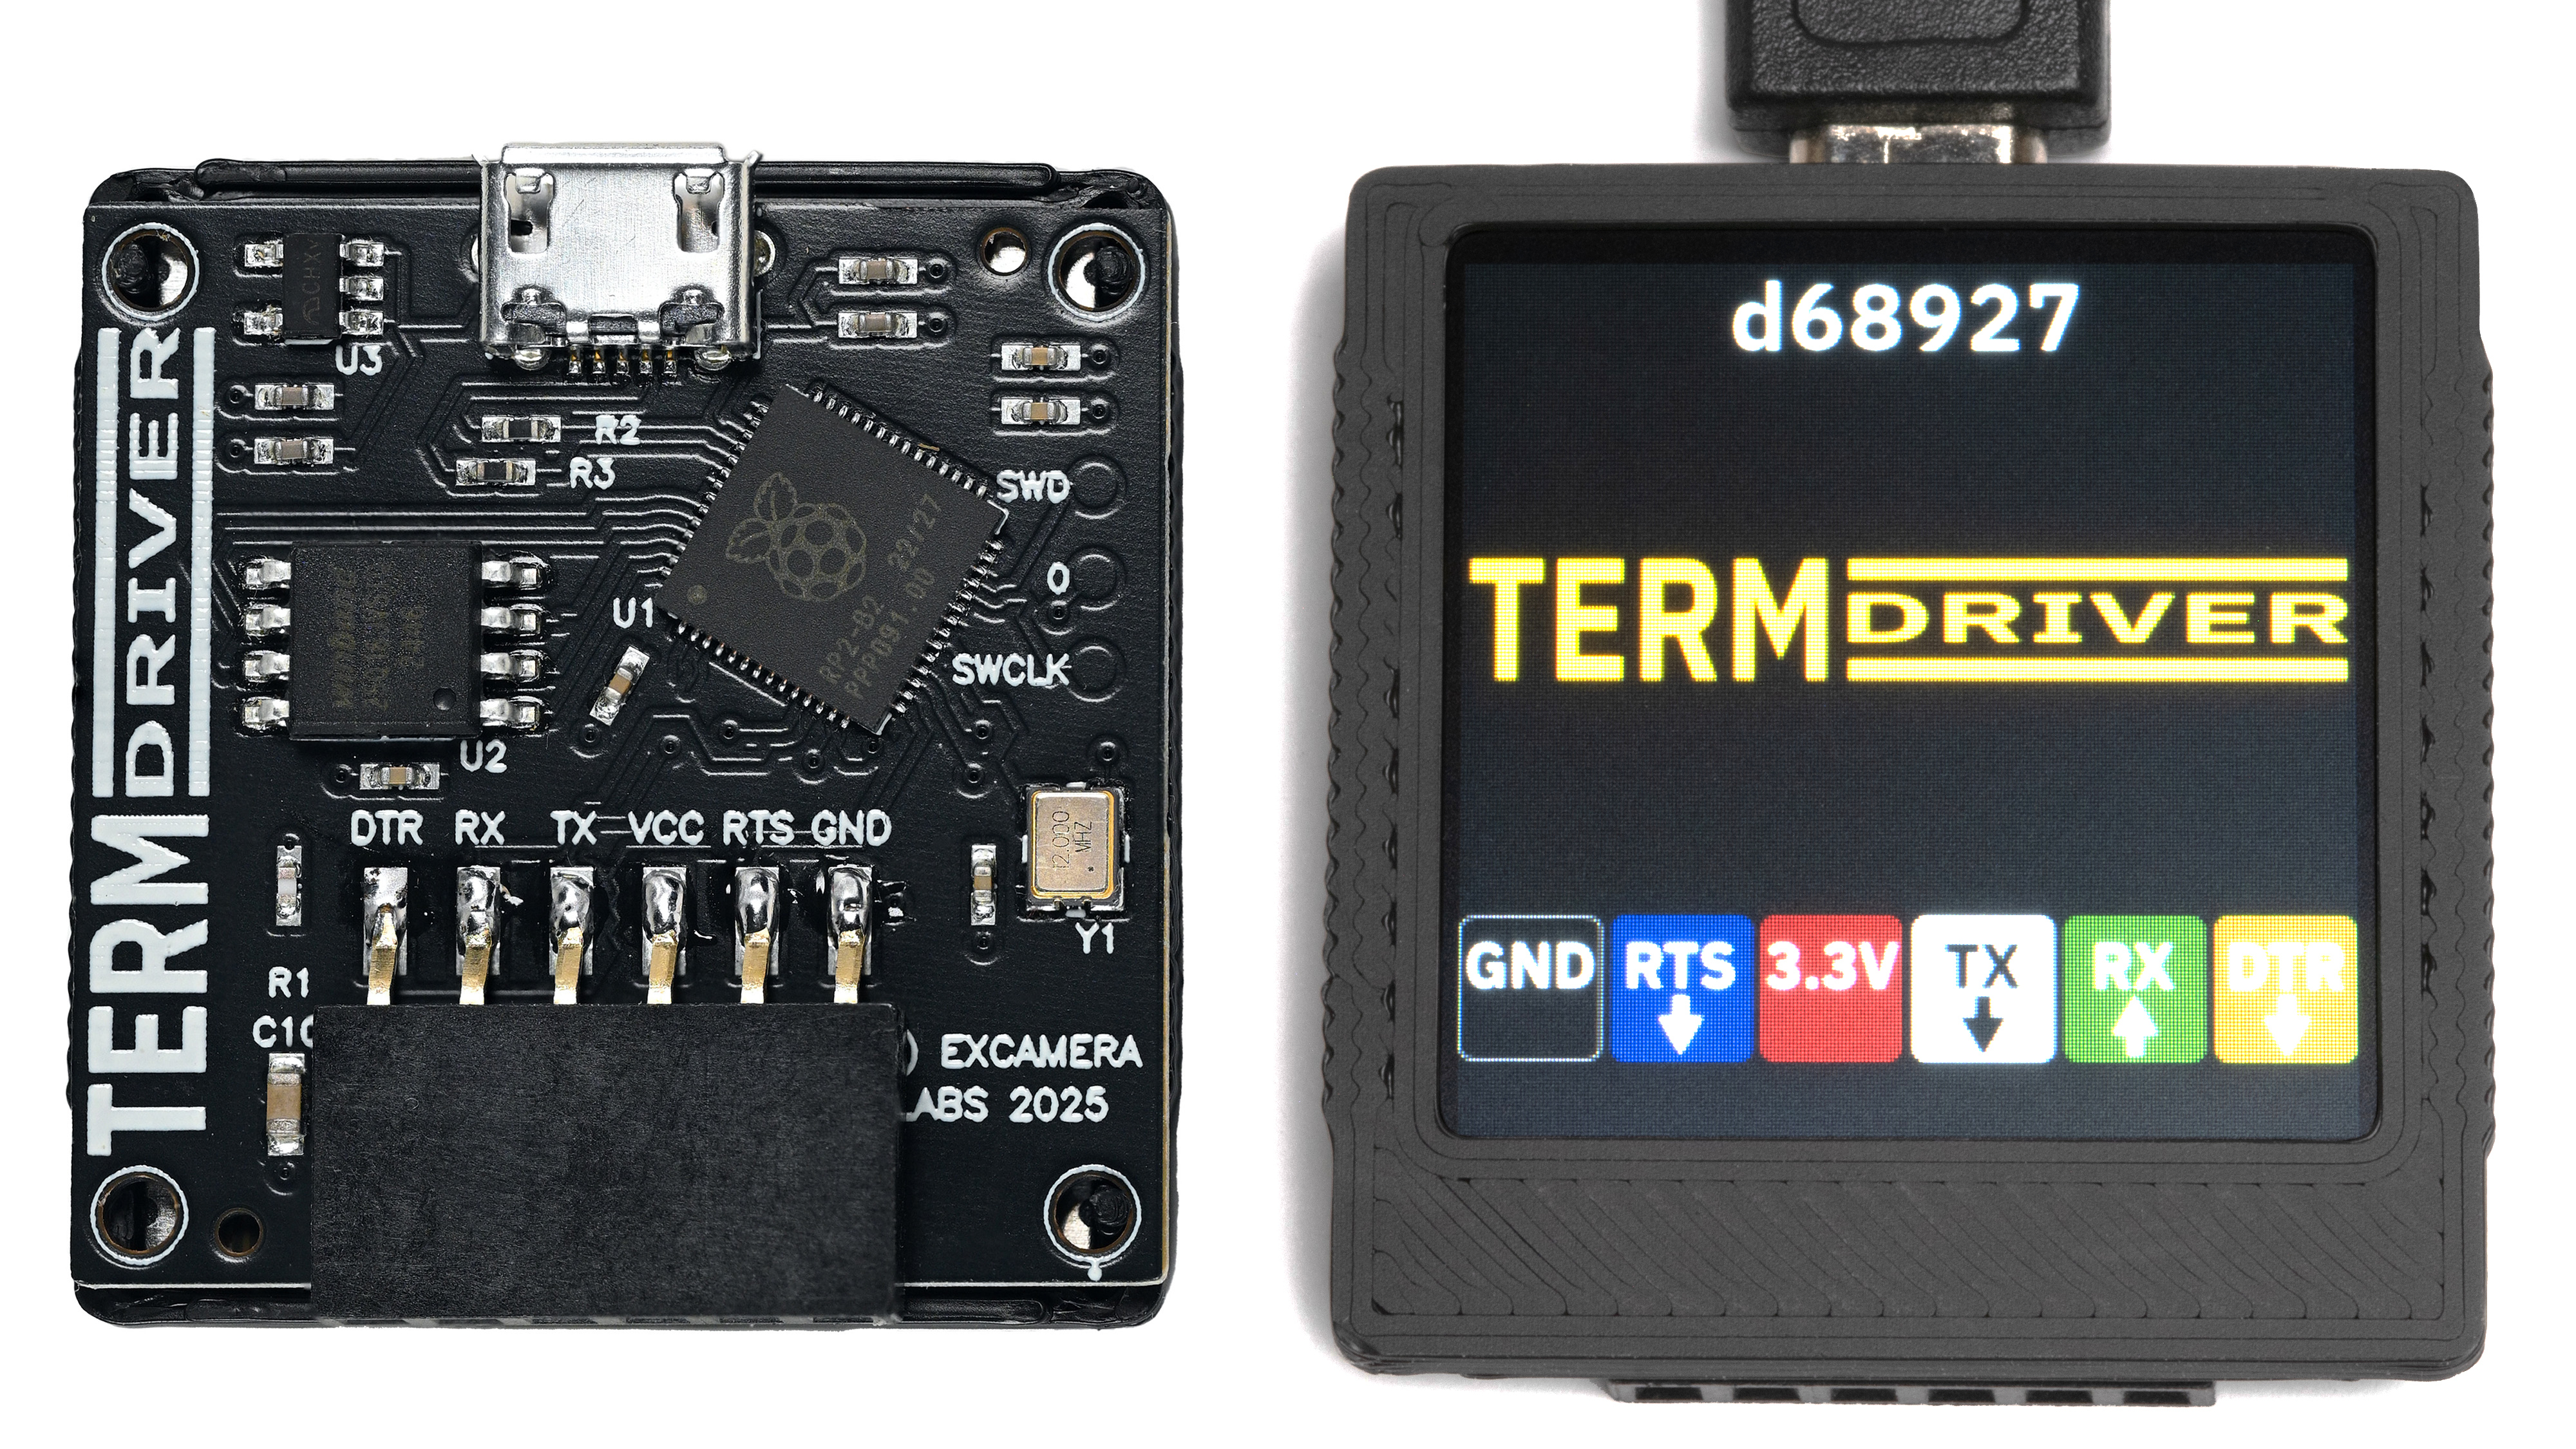
\includegraphics[width=0.75\textwidth]{img/termdriver2/termdriver2-front-back-01-comp}
\end{center}

TermDriver2 has 6 output pins, on a standard 2.54 mm (0.1") female header.

\gap
\noindent
\begin{tabularx}{\linewidth}{lllX}
Pin & Signal & Function & Notes \\ \heavyline \\

1 & GND  & power  & Ground \\
2 & RTS  & output & Request to send \index{CTS} \\
3 & 3.3V & power  & Up to 300 mA available \\
4 & TX   & output & Data transmit \\
5 & RX   & input  & Data receive \\
6 & DTR  & output & Data terminal ready, output \index{DTR}\\

\\ \heavyline
\end{tabularx}
\gap

\subsection{Standalone mode}

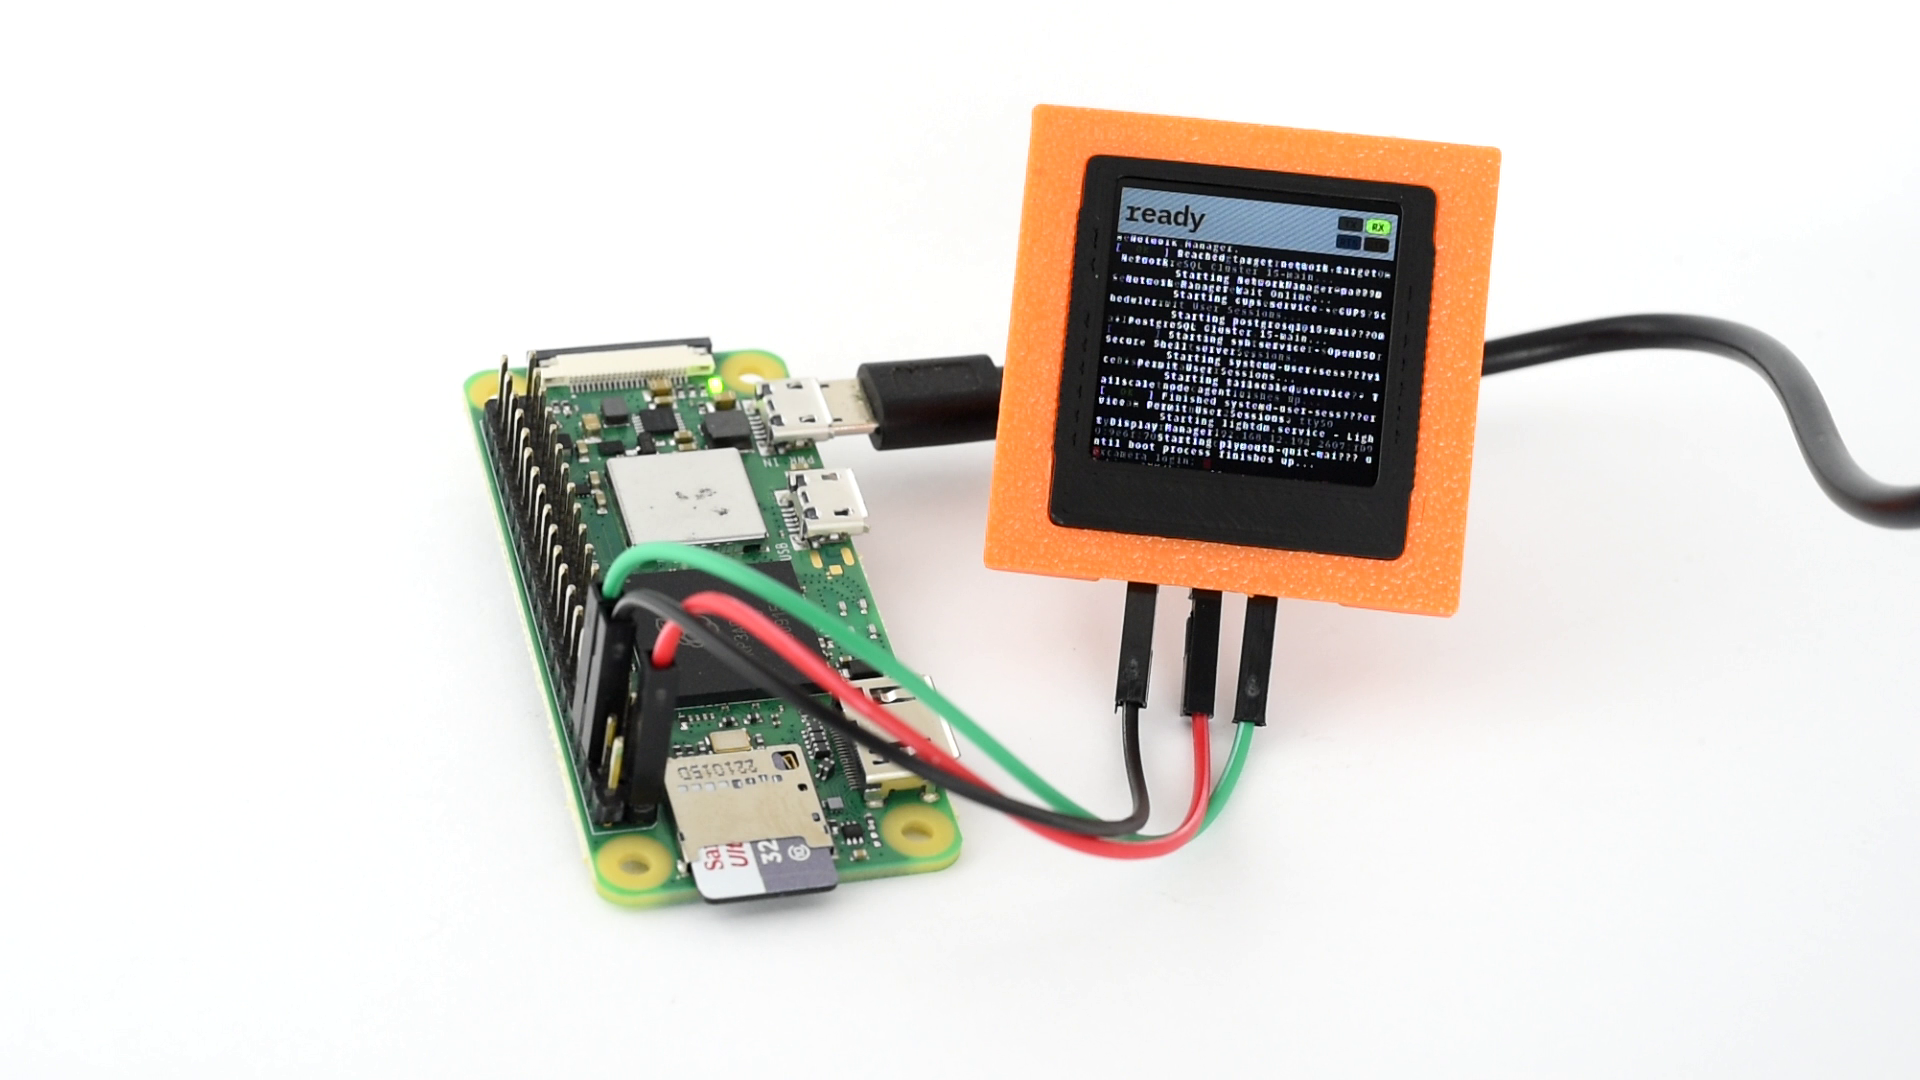
\includegraphics[width=0.75\textwidth]{img/termdriver2/shot0003}

In addition to working as a USB powered peripheral,
TermDriver can run in standalone mode with no USB connection.
In this mode 3.3 V power is supplied by the target circuit.
Connect GND, 3.3V and RX to the target circuit.

When running in standalone mode, TermDriver's line configuration is 115200 8N1.

\subsection{Internals}

The onboard RP2040 microcontroller runs at 125 MHz,
and has 2 Mbyte of program flash.

The display is a ST7789 controller with a 240x240 panel.

The RP2040 has these GPIO connections.

\gap
\begin{tabular}{lcl}
Signal & GPIO & \\
\hline \\
\mach{UART\_TX\_PIN} &  8 &  external pin 4         \\
\mach{UART\_RX\_PIN} &  9 &  external pin 5         \\
\mach{DTR\_PIN}      & 12 &  external pin 6         \\
\mach{RTS\_PIN}      & 13 &  external pin 2         \\
\mach{PIN\_SCK}      & 14 &  panel clock            \\
\mach{PIN\_MOSI}     & 15 &  panel data             \\
\mach{PIN\_RES}      & 11 &  panel reset            \\
\mach{PIN\_DC}       & 10 &  panel command/data     \\
\hline \\
\end{tabular}

\section{Specifications}

\subsection{DC characteristics}
\vspace{10 pt}
{\renewcommand{\arraystretch}{1.2}% for the vertical padding

\begin{tabularx}{\linewidth}{XC{40pt}C{40pt}C{40pt}C{40pt}}
\heavyline
& min & typ & max & units \\ \heavyline

RX & & & & \\
\hspace{10pt}low voltage & 0 & & 0.6 & V \\
\hspace{10pt}high voltage & 2.7 &   & 3.3 & V     \\ \hline
Output signal current (TX, RTS, DTR)  &&& 4 & mA  \\ \hline
Output voltage        & & 3.3 & & V               \\ \hline
Output current        & & 330 & & mA              \\ \hline
Current consumption   & & 25 & & mA               \\ \hline

\end{tabularx}}
\vspace{10 pt}

\subsection{AC characteristics}
\vspace{10 pt}

{\renewcommand{\arraystretch}{1.2}% for the vertical padding
\begin{tabularx}{\linewidth}{XC{40pt}C{40pt}C{40pt}C{40pt}}
\heavyline
& min & typ & max & units \\ \heavyline

UART speed                     &110& &2M& bps   \index{speed!UART}\\ \hline
Startup time & & & 100 & ms \\ \hline
\end{tabularx}}
\vspace{10 pt}

\section{Troubleshooting}

\gap
\begin{tabular}{|l|l|}
\hline
Screen is dark after connecting USB  & Check USB cable and port \\
                                     & Return for replacement \\
\hline
Screen is white after connecting USB & Return for replacement \\
\hline
Port does not appear on host         & Check that the USB Cable is not "power only" \\
                                     & Check USB cable and port \\
                                     & Return for replacement \\
\hline
\end{tabular}
\gap

\section{Support information}

Technical and product support is available at
\href{mailto:support@termdriver.com}{support@termdriver.com}

TermDriver2 is built and maintained by
\href{https://excamera.com}{Excamera Labs}.

\newpage
\raggedright
\addcontentsline{toc}{section}{Index}
\renewcommand{\indexname}{Index}
\printindex

\end{document}
